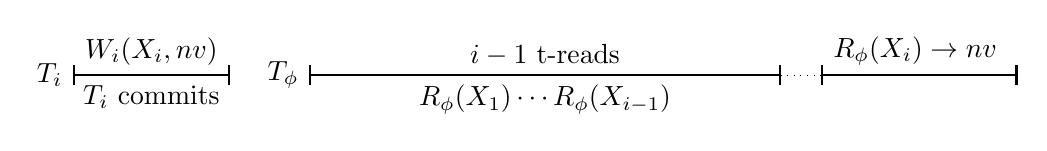
\begin{tikzpicture}
\node (r1) at (3,0) [] {};
\node (r2) at (7.7,0) [] {};

\node (w1) at (-2,0) [] {};


\draw (r1) node [below] {\normalsize {$R_{\phi}(X_1) \cdots R_{\phi}(X_{i-1})$}};
\draw (r1) node [above] {\normalsize {$i-1$ t-reads}};

\draw (r2) node [above] {\normalsize {$R_{\phi}(X_i)\rightarrow nv$}};

\draw (w1) node [above] {\normalsize {$W_i(X_i,nv)$}}; 
\draw (w1) node [below] {\normalsize {$T_i$ commits}};


\begin{scope}   
\draw [|-|,thick] (0,0) node[left] {$T_{\phi}$} to (6,0);
\draw [|-|,thick] (6.5,0) node[left] {} to (9,0);
\draw [-,dotted] (0,0) node[left] {} to (9,0);
\end{scope}
%
%
\begin{scope}   
%\draw [|-|,thick] (0,0) node[left] {$T_k$} to (6,0);
\draw [|-|,thick] (-3,0) node[left] {$T_i$} to (-1,0);
\end{scope}
%
\end{tikzpicture}
